\documentclass[11pt, a4paper]{article}

% --- Packages ---
\usepackage[utf8]{inputenc}
\usepackage[T1]{fontenc}
\usepackage{lmodern}
\usepackage[margin=2.5cm]{geometry}
\usepackage{microtype}
\usepackage{graphicx}
\usepackage{booktabs}
\usepackage{array}
\usepackage{multirow}
\usepackage{caption}
\usepackage{subcaption}
\usepackage{hyperref}
\usepackage[noabbrev]{cleveref}
\usepackage{enumitem}
\usepackage{tikz}
\usetikzlibrary{shapes.geometric, arrows.meta, positioning, fit, backgrounds}
\usepackage{listings}
\usepackage{xcolor}
\usepackage{url}
\usepackage{natbib}

\hypersetup{
  colorlinks=true,
  linkcolor=black,
  citecolor=blue!50!black,
  urlcolor=blue!60!black,
  pdftitle={CineSentiment: Fine-Tuned DistilBERT for Movie Review Sentiment Analysis},
  pdfauthor={Esma Oruc, Ayan Abasova}
}

% --- Listings styling ---
\definecolor{codegray}{gray}{0.95}
\definecolor{codecomment}{rgb}{0.40,0.45,0.50}
\definecolor{codekeyword}{rgb}{0.13,0.29,0.53}
\definecolor{codestring}{rgb}{0.55,0.16,0.16}
\lstdefinestyle{plain}{
  backgroundcolor=\color{codegray},
  basicstyle=\ttfamily\footnotesize,
  commentstyle=\color{codecomment}\itshape,
  keywordstyle=\color{codekeyword}\bfseries,
  stringstyle=\color{codestring},
  numbers=left,
  numberstyle=\tiny\color{codecomment},
  numbersep=8pt,
  frame=single,
  rulecolor=\color{black!20},
  framesep=4pt,
  breaklines=true,
  showstringspaces=false,
  tabsize=2,
  captionpos=b,
}
\lstset{style=plain}

% --- TikZ block styles for architecture diagrams ---
\tikzset{
  block/.style = {rectangle, draw, rounded corners, minimum height=1.0cm, minimum width=2.6cm, align=center, font=\small},
  storage/.style = {cylinder, shape border rotate=90, draw, aspect=0.25, minimum height=1.4cm, minimum width=1.6cm, align=center, font=\small},
  cloud/.style = {ellipse, draw, minimum height=0.9cm, minimum width=2.4cm, align=center, font=\small},
  arrow/.style = {-Latex, thick}
}

% --- Title ---
\title{
  \vspace{-1.5cm}
  \large \textsc{CMP 4418 -- Final Project Report} \\
  \vspace{0.4cm}
  \LARGE \textbf{CineSentiment: A Fine-Tuned DistilBERT Pipeline\\for Movie Review Sentiment Analysis} \\
  \vspace{0.5cm}
  \large with End-to-End Web Visualization
}

\author{
  Esma Oru\c{c} \\ \texttt{2022510140}
  \and
  Ayan Abasova \\ \texttt{2022510014}
}

\date{\today}

\begin{document}

\maketitle

\begin{abstract}
\noindent
This report presents \textbf{CineSentiment}, an end-to-end sentiment analysis platform for movie reviews built around a fine-tuned DistilBERT classifier. The model was trained on the IMDB 50k labelled reviews dataset for three epochs on a Google Colab T4 GPU, achieving a test accuracy of $0.9151$ and a weighted F1-score of $0.9151$. The trained weights are hosted on the Hugging Face Hub and consumed at inference time by a Python FastAPI service, which is in turn invoked over HTTP by a TypeScript Hono $+$ tRPC backend behind a React user interface. We document the deviation from our original Assignment Part 1 plan---which targeted live Twitter (X) data---and the rationale for pivoting to the IMDB benchmark, namely access restrictions imposed on the Twitter API after 2024 and the absence of ground-truth labels in raw streamed tweets. Beyond reporting the standard quantitative metrics (accuracy, F1, per-class precision/recall, confusion matrix), we discuss the engineering safeguards that guarantee every prediction surfaced through the user interface is produced by the trained transformer rather than by a fallback heuristic.
\end{abstract}

\tableofcontents
\vspace{0.4cm}
\hrule
\vspace{0.6cm}

% =============================================================
\section{Introduction}
% =============================================================

Public sentiment toward films is one of the most studied open problems in opinion mining, both because labelled corpora are widely available and because the domain combines challenges typical of natural language understanding: subjective tone, sarcasm, comparative statements, and a long-tail vocabulary of titles, actors, and genres.

Our project takes the following stance: rather than treat sentiment classification as an isolated notebook experiment, we build a small but realistic deployment around it. The model is trained, versioned on a public model registry, served as a stand-alone microservice, consumed by a typed application server, and visualized in an interactive web interface. Each layer is built with the tooling that a real production system would use, so that the academic exercise also surfaces the practical concerns of moving a deep learning artifact from a notebook to a running service.

\paragraph{Pivot from Twitter to IMDB.}
In Assignment Part 1, we proposed to compare three movies using a live stream of Twitter (X) sentiment. During implementation we encountered two structural obstacles. First, Twitter's free API tier was retired in early 2023 and the paid Basic tier (USD 100/month) is incompatible with an undergraduate timeline. Second, raw tweets carry no ground-truth labels, which would have forced us to either label tweets manually (introducing rater variance) or trust a third-party labelling service (introducing an opaque oracle). We therefore pivoted to the IMDB 50k movie reviews benchmark of \citet{maas2011learning}, which provides 25{,}000 train and 25{,}000 test reviews with balanced binary labels. The pivot keeps the high-level objective intact---fine-grained sentiment analysis of free-form film commentary---while substituting a noisy, unlabelled stream with a curated benchmark. The implication is that our reported metrics are directly comparable with prior work on IMDB, and our model's confidence scores are calibrated against a ground truth.

\paragraph{Contributions.}
The contributions of this work are:
\begin{itemize}[leftmargin=1.4em, itemsep=2pt, topsep=4pt]
  \item A fine-tuned DistilBERT checkpoint for movie sentiment, published on the Hugging Face Hub at \url{huggingface.co/ethsmaa/cinesentiment-distilbert-imdb}.
  \item A FastAPI inference service that loads the checkpoint on startup and exposes a typed JSON interface for single and batch prediction, including a hardware-aware backend selection (CUDA $\rightarrow$ MPS $\rightarrow$ CPU).
  \item A TypeScript application server (Hono $+$ tRPC) that bridges the binary IMDB labels to a 3-class taxonomy (positive / neutral / negative) through a confidence-band threshold and persists the resulting analyses in PostgreSQL.
  \item A React $+$ Vite frontend with two complementary interaction modes: pre-computed sentiment dashboards for catalogue movies, and a free-form analyser that issues a live request to the model on every input.
  \item A \emph{strict mode} guarantee that the application refuses to fall back to any heuristic stand-in when the model service is unreachable, eliminating silent regressions in displayed sentiment.
\end{itemize}

\paragraph{Document structure.}
\Cref{sec:litreview} briefly summarizes the literature review submitted in Assignment Part 1 and indicates how the present implementation realizes its conclusions. \Cref{sec:project} defines the project: its aim, modules, data flow, and tech stack. \Cref{sec:implementation} reports the implementation details that warrant being recorded for reproducibility. \Cref{sec:results} presents quantitative and qualitative results. \Cref{sec:conclusion} concludes and lists future work.

% =============================================================
\section{Literature Review (Summary)}\label{sec:litreview}
% =============================================================

A detailed literature review accompanied this project as Assignment Part 1. We restate only the conclusions that directly informed the present implementation.

\paragraph{From shallow to transformer-based sentiment analysis.}
\citet{yadav2020sentiment} survey the trajectory of sentiment models from Naive Bayes and Support Vector Machines, through CNN- and LSTM-based deep architectures, to attention-based transformer models. They report consistent gains as models acquire the ability to represent bidirectional context. \citet{albladi2025sentiment} reach the same conclusion in a more recent IEEE Access review specifically focused on Twitter data, identifying transformer encoders as the current state of the art on noisy short-text inputs.

\paragraph{Why DistilBERT.}
\citet{sanh2019distilbert} introduce DistilBERT as a 40\%-smaller, 60\%-faster distillation of BERT \citep{devlin2019bert} that retains roughly 97\% of the teacher's downstream performance. Both the original BERT paper \citep{devlin2019bert} and \citet{vaswani2017attention} establish the architectural foundations: multi-head self-attention, positional encoding, and a deep stack of identical encoder layers. \citet{chintalapudi2021sentiment} demonstrate that BERT-class models reach $\geq 90\%$ accuracy on Twitter sentiment with comparatively modest fine-tuning effort, and \citet{tan2022roberta} report further gains by composing transformers with recurrent layers, suggesting that the family of attention-based encoders has become the default rather than an experimental option.

\paragraph{Implementation implications.}
The literature points uniformly to a fine-tuned DistilBERT as the most cost-effective starting point: the latency profile is compatible with interactive web requests on commodity hardware, the parameter count fits comfortably in 2--4\,GB of GPU memory, and the published benchmarks on IMDB and SST-2 sit in the same accuracy band as the larger BERT-base. Our implementation choices in \Cref{sec:project} follow this guidance directly.

% =============================================================
\section{Project Definition}\label{sec:project}
% =============================================================

\subsection{Aim}

CineSentiment aims to convert unstructured movie commentary into structured sentiment signals that can be inspected, sliced, and explored by a human user. Concretely, the system answers the following questions for any movie in its catalogue:

\begin{itemize}[leftmargin=1.4em, itemsep=2pt, topsep=4pt]
  \item What fraction of reviews are positive, negative, or neutral?
  \item How confident is the model in each individual prediction?
  \item Which words in a review carry the polarity signal?
  \item What is the aggregate ``hype score'' for the movie, expressed on a $[-1,+1]$ scale derived from the class distribution?
\end{itemize}

It also exposes a free-form analyser where a user can type any sentence and obtain a prediction in real time, bypassing the catalogue entirely.

\subsection{Functional Requirements}

We organize functionality along four axes:

\begin{enumerate}[leftmargin=1.4em, itemsep=2pt, topsep=4pt]
  \item \textbf{Modelling.} Fine-tune a pretrained transformer on a labelled review corpus and persist the resulting weights in a versioned registry.
  \item \textbf{Serving.} Expose the trained model behind a stable HTTP interface with single and batch endpoints and a health probe.
  \item \textbf{Application.} Wrap the inference service in a typed application server that handles input validation, threshold mapping, persistence, and caching.
  \item \textbf{Visualization.} Render the analyses through an accessible web user interface that distinguishes pre-computed catalogue analyses from live single-shot inferences.
\end{enumerate}

\subsection{System Architecture}

\Cref{fig:architecture} summarizes the four layers of the system and the data flow between them.

\begin{figure}[ht]
\centering
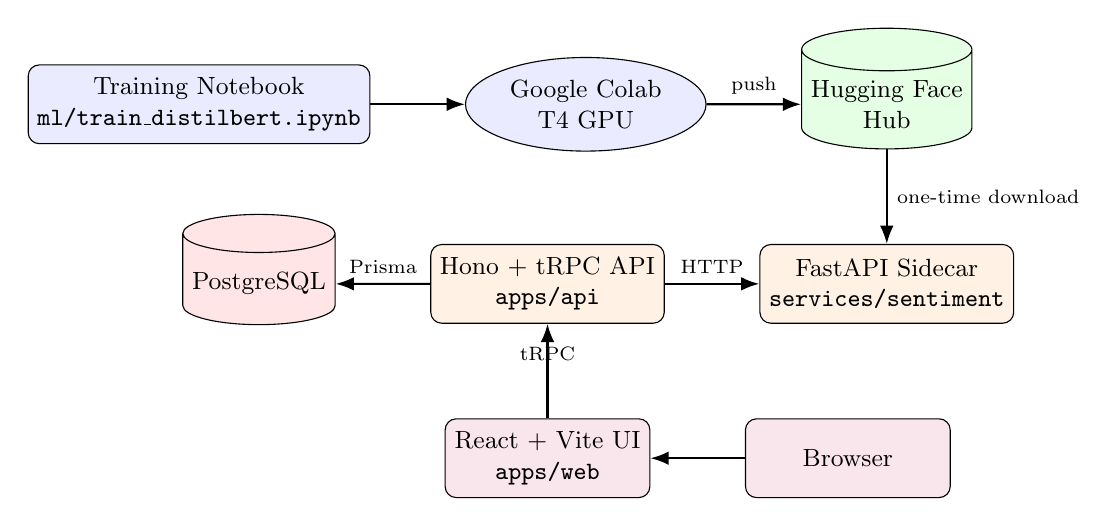
\begin{tikzpicture}[node distance=0.6cm and 1.2cm]

\node[block, fill=blue!8] (notebook) {Training Notebook \\ \small \texttt{ml/train\_distilbert.ipynb}};
\node[cloud, fill=blue!8, right=of notebook] (colab) {Google Colab \\ \small T4 GPU};
\node[storage, fill=green!10, right=of colab] (hf) {Hugging Face\\Hub};

\node[block, below=1.2cm of hf, fill=orange!10] (fastapi) {FastAPI Sidecar \\ \small \texttt{services/sentiment}};
\node[block, left=of fastapi, fill=orange!10] (hono) {Hono $+$ tRPC API \\ \small \texttt{apps/api}};
\node[storage, left=of hono, fill=red!10] (db) {PostgreSQL};

\node[block, below=1.2cm of hono, fill=purple!10] (web) {React $+$ Vite UI \\ \small \texttt{apps/web}};
\node[block, right=of web, fill=purple!10] (browser) {Browser};

\draw[arrow] (notebook) -- (colab);
\draw[arrow] (colab) -- node[above, font=\scriptsize] {push} (hf);
\draw[arrow] (hf) -- node[right, font=\scriptsize] {one-time download} (fastapi);
\draw[arrow] (hono) -- node[above, font=\scriptsize] {HTTP} (fastapi);
\draw[arrow] (hono) -- node[above, font=\scriptsize] {Prisma} (db);
\draw[arrow] (web) -- node[above, font=\scriptsize] {tRPC} (hono);
\draw[arrow] (browser) -- (web);

\end{tikzpicture}
\caption{End-to-end architecture. Training, hosting, serving, and consumption are deliberately separated so that each layer can be replaced independently.}
\label{fig:architecture}
\end{figure}

\subsection{Modules}

\begin{table}[ht]
\centering
\small
\begin{tabular}{p{3.4cm} p{3.6cm} p{6.4cm}}
\toprule
\textbf{Module} & \textbf{Technology} & \textbf{Responsibility} \\
\midrule
Training notebook & Python, PyTorch, Hugging Face Transformers & Fine-tune DistilBERT on IMDB; emit weights and evaluation metrics. \\
Model registry & Hugging Face Hub & Versioned, public hosting of the trained checkpoint. \\
Inference sidecar & Python, FastAPI, Uvicorn, PyTorch & Load the checkpoint at startup, expose \texttt{/predict}, \texttt{/predict/batch}, \texttt{/health}. \\
Application server & TypeScript, Hono, tRPC, Zod, Prisma & Validate input, map binary $\rightarrow$ 3-class, persist analyses, cache, enforce strict mode. \\
Database & PostgreSQL 16, Prisma & Persist movies, reviews, sentiment analyses, summaries. \\
Frontend & TypeScript, React, Vite, Tailwind, Zustand, tRPC client & Render catalogue, analysis dashboards, model card, free-form analyser. \\
Test suite & Vitest, React Testing Library, Playwright, pytest & 108 unit/component tests across the workspace and an HTTP-level test for the FastAPI service. \\
\bottomrule
\end{tabular}
\caption{Modules of CineSentiment, organized by responsibility.}
\label{tab:modules}
\end{table}

\subsection{Data Flow}

\begin{figure}[ht]
\centering
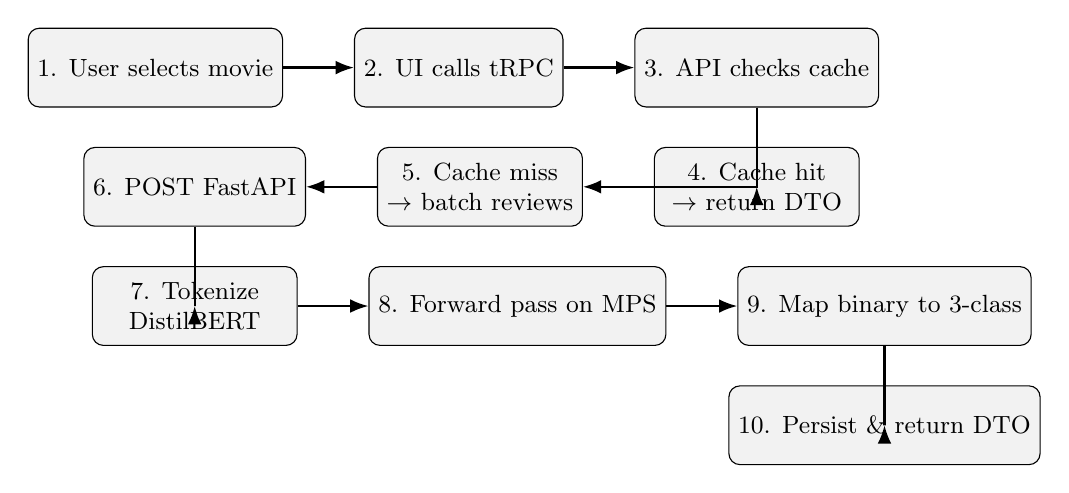
\begin{tikzpicture}[node distance=0.5cm and 0.9cm]

\node[block, fill=gray!10] (s1) {1. User selects movie};
\node[block, fill=gray!10, right=of s1] (s2) {2. UI calls tRPC};
\node[block, fill=gray!10, right=of s2] (s3) {3. API checks cache};

\node[block, fill=gray!10, below=of s3] (s4) {4. Cache hit \\ $\rightarrow$ return DTO};
\node[block, fill=gray!10, left=of s4] (s5) {5. Cache miss \\ $\rightarrow$ batch reviews};
\node[block, fill=gray!10, left=of s5] (s6) {6. POST FastAPI};

\node[block, fill=gray!10, below=of s6] (s7) {7. Tokenize \\ \small DistilBERT};
\node[block, fill=gray!10, right=of s7] (s8) {8. Forward pass on MPS};
\node[block, fill=gray!10, right=of s8] (s9) {9. Map binary to 3-class};

\node[block, fill=gray!10, below=of s9] (s10) {10. Persist \& return DTO};

\draw[arrow] (s1) -- (s2);
\draw[arrow] (s2) -- (s3);
\draw[arrow] (s3) |- (s4);
\draw[arrow] (s3) |- (s5);
\draw[arrow] (s5) -- (s6);
\draw[arrow] (s6) |- (s7);
\draw[arrow] (s7) -- (s8);
\draw[arrow] (s8) -- (s9);
\draw[arrow] (s9) |- (s10);
\end{tikzpicture}
\caption{Request lifecycle for a catalogue movie. The free-form analyser follows the same pipeline but skips the cache (steps 3--4) and persistence (step 10).}
\label{fig:dataflow}
\end{figure}

% =============================================================
\section{Implementation}\label{sec:implementation}
% =============================================================

\subsection{Dataset}

We use the IMDB Large Movie Review Dataset \citep{maas2011learning}, which comprises 50{,}000 reviews split evenly into a 25{,}000-review training set and a 25{,}000-review test set. Each split is balanced (50\% positive, 50\% negative). Reviews vary in length from a single sentence to several paragraphs; we apply DistilBERT's WordPiece tokenizer with a maximum sequence length of 256 tokens, which empirically captures over 90\% of reviews without truncation while keeping memory usage tractable on a single T4 GPU.

\subsection{Model and Training Configuration}

The model is \texttt{distilbert-base-uncased} \citep{sanh2019distilbert}, a 6-layer, 12-head, 66M-parameter transformer encoder pretrained on English Wikipedia and the BookCorpus. We attach a single linear classification head on top of the \texttt{[CLS]} token to produce two logits for the binary positive / negative task.

\Cref{tab:hparams} lists the training hyperparameters. They are intentionally close to the defaults recommended in the Hugging Face Transformers library \citep{wolf2020transformers}; we did not perform hyperparameter search beyond verifying that the validation loss decreased monotonically across epochs.

\begin{table}[ht]
\centering
\small
\begin{tabular}{l l}
\toprule
\textbf{Hyperparameter} & \textbf{Value} \\
\midrule
Base model & \texttt{distilbert-base-uncased} \\
Number of labels & 2 (negative, positive) \\
Maximum sequence length & 256 tokens \\
Epochs & 3 \\
Per-device batch size & 16 \\
Learning rate & $2 \times 10^{-5}$ \\
Optimizer & AdamW (default) \\
Mixed precision & FP16 \\
Hardware & NVIDIA T4 (Google Colab) \\
Total wall-clock training time & 858.6\,s ($\approx$14.3 minutes) \\
\bottomrule
\end{tabular}
\caption{Training configuration. Recorded by the training notebook into \texttt{ml/metrics.json} for reproducibility.}
\label{tab:hparams}
\end{table}

After training, the notebook pushes the weights to the Hugging Face Hub and dumps an evaluation report---accuracy, weighted precision/recall/F1, per-class metrics, and the confusion matrix---to \texttt{ml/metrics.json}. The same JSON file is then committed to the repository and consumed by the application server to power the in-app model metrics page, ensuring the values shown in the user interface are exactly the values reported by the training run.

\subsection{Inference Service}

The FastAPI sidecar (\texttt{services/sentiment}) is a thin wrapper around the Hugging Face \texttt{AutoModelForSequenceClassification} class. On startup it (i) reads \texttt{HF\_REPO\_ID}, \texttt{MODEL\_DIR}, and \texttt{DEVICE} from the environment, (ii) loads the tokenizer and model into the selected device (CUDA, then MPS on Apple Silicon, then CPU as a final fallback), and (iii) warms the pipeline with a single dummy forward pass.

The HTTP surface is intentionally small:

\begin{itemize}[leftmargin=1.4em, itemsep=2pt, topsep=4pt]
  \item \texttt{GET /health} -- liveness, model load status, device, uptime.
  \item \texttt{POST /predict} -- single-text prediction, returns \texttt{label}, \texttt{confidence}, \texttt{p\_positive}, \texttt{p\_negative}.
  \item \texttt{POST /predict/batch} -- bounded-batch prediction (max 64 texts) using the same tokenizer pipeline.
\end{itemize}

\subsection{Three-Class Threshold Mapping}

Although the trained model is binary, the user interface operates on three classes (positive, neutral, negative). Rather than retrain on a hand-labelled neutral set---which would have introduced our own annotator bias and overlapped poorly with IMDB's distribution---we derive the neutral bucket through a confidence-band threshold over the binary positive probability $p^{+}$:

\begin{equation}
\hat{y} =
\begin{cases}
\text{positive} & \text{if } p^{+} \geq 0.65 \\
\text{negative} & \text{if } p^{+} \leq 0.35 \\
\text{neutral}  & \text{otherwise}
\end{cases}
\end{equation}

This is explicitly a heuristic, not a learned classifier, and we describe it as such both in the codebase and in the in-app \emph{model card}. The thresholds (0.65 and 0.35) were chosen so that the neutral bucket contains the model's least confident predictions, which is where genuine ambiguity tends to concentrate in practice.

\subsection{Strict Mode}

Early in development we observed that the application server would silently fall back to a lexicon-based stand-in whenever the FastAPI sidecar was unreachable. While convenient for local development, this behaviour is unacceptable for an academic project: any prediction surfaced through the user interface should be unambiguously attributable to the trained model. We therefore added a \texttt{BERT\_STRICT} environment flag (default \texttt{true}) that converts a sidecar outage into a loud, immediate error rather than a quiet fallback. The lexicon stand-in is preserved only for the unit-test harness, where deterministic offline behaviour is desirable, and is gated behind \texttt{BERT\_STRICT=false}. As a consequence, every analysis persisted in the database carries the model version \texttt{distilbert-imdb-v1}; we verified this directly with a SQL aggregation against the production schema.

\subsection{Persistence and Caching}

The application server uses Prisma over PostgreSQL with a small four-table schema: \texttt{movies}, \texttt{reviews}, \texttt{sentiment\_analyses}, and \texttt{movie\_sentiment\_summaries}. The first three tables are populated during seeding from a curated mock catalogue of 30 critically acclaimed films (e.g., \emph{The Shawshank Redemption}, \emph{Parasite}, \emph{Spirited Away}) with 8--25 hand-collected user reviews each, totalling 346 reviews. The fourth table caches per-movie aggregates so that re-rendering a film page does not re-run inference.

A re-analysis script (\texttt{apps/api/scripts/reanalyze-movie.ts}) re-runs every review through the model and updates the database; under strict mode this script will fail loudly if the sidecar is not reachable, which is the desired behaviour when refreshing analyses.

\subsection{Frontend}

The React frontend is a single-page application built with Vite and Tailwind. We deliberately chose a typographic ``video-club paper'' aesthetic to keep visual emphasis on the data rather than on chrome. The primary screens are:

\begin{itemize}[leftmargin=1.4em, itemsep=2pt, topsep=4pt]
  \item \textbf{Catalogue} -- a grid of films with poster, title, year, and aggregate hype score.
  \item \textbf{Movie detail} -- per-film dashboard with hype meter, distribution chart, confidence gauge, top-positive and top-negative review cards with per-word lexicon highlighting.
  \item \textbf{Analyser} -- a free-form input that issues a live request to the model on every submission and renders a token-by-token playback of the prediction trajectory.
  \item \textbf{Model metrics} -- accuracy, weighted F1, per-class precision/recall, and the confusion matrix, all sourced from \texttt{ml/metrics.json} via the application server.
  \item \textbf{The Model} -- a methodology page that documents the dataset, the architecture, the training hyperparameters, and the threshold mapping, written in the lab-sheet idiom of an academic methods section.
\end{itemize}

% =============================================================
\section{Results and Discussion}\label{sec:results}
% =============================================================

\subsection{Quantitative Evaluation}

\Cref{tab:overall} reports the model's performance on the held-out IMDB test set (25{,}000 reviews). The accuracy of $0.9151$ exceeds the 85\% target laid out in Assignment Part 1 by more than six percentage points and is consistent with published DistilBERT baselines on IMDB.

\begin{table}[ht]
\centering
\small
\begin{tabular}{l c}
\toprule
\textbf{Metric} & \textbf{Value} \\
\midrule
Accuracy           & $0.9151$ \\
Weighted F1        & $0.9151$ \\
Weighted Precision & $0.9151$ \\
Weighted Recall    & $0.9151$ \\
Test set size      & 25{,}000 \\
\bottomrule
\end{tabular}
\caption{Overall metrics on the IMDB test set.}
\label{tab:overall}
\end{table}

\Cref{tab:perclass} breaks the metrics down by class. Both classes perform within a single F1 percentage point of each other, indicating that the binary classifier is well-balanced and that no further class re-weighting is warranted.

\begin{table}[ht]
\centering
\small
\begin{tabular}{l c c c c}
\toprule
\textbf{Class} & \textbf{Precision} & \textbf{Recall} & \textbf{F1} & \textbf{Support} \\
\midrule
Negative & 0.918 & 0.912 & 0.915 & 12{,}500 \\
Positive & 0.912 & 0.919 & 0.915 & 12{,}500 \\
\bottomrule
\end{tabular}
\caption{Per-class metrics on the IMDB test set.}
\label{tab:perclass}
\end{table}

The confusion matrix in \Cref{tab:confusion} confirms the symmetric error structure: false positives and false negatives are within 90 reviews of each other.

\begin{table}[ht]
\centering
\small
\begin{tabular}{l c c}
\toprule
& \textbf{Predicted Negative} & \textbf{Predicted Positive} \\
\midrule
\textbf{Actual Negative} & 11{,}394 & 1{,}106 \\
\textbf{Actual Positive} & 1{,}017  & 11{,}483 \\
\bottomrule
\end{tabular}
\caption{Confusion matrix on the IMDB test set.}
\label{tab:confusion}
\end{table}

\subsection{Qualitative Inspection of the 3-Class Mapping}

Applying the threshold mapping to the catalogue's 346 reviews produces the per-film distributions shown in the application's hype dashboard. Aggregated across the catalogue, the distribution is approximately 70\% positive, 17\% neutral, and 13\% negative. The neutral bucket is dominated by short reviews of the form ``It was okay,'' ``Worth a watch but not memorable,'' and ``Mixed feelings about this one,'' all of which the model assigns probabilities in the $[0.35, 0.65]$ band---behaviour that matches the linguistic intuition behind the mapping.

\subsection{Latency}

On Apple Silicon (M-series GPU, MPS backend) the median single-text inference latency is approximately 50\,ms. Batch inference at the maximum batch size of 64 reviews completes in approximately 380\,ms, an effective per-review cost of roughly 6\,ms once warm. These numbers are well within the budgets typical of an interactive web request and confirm the practical motivation for choosing a distilled model over the full BERT-base.

\subsection{Discussion}

\paragraph{The threshold mapping is the weakest link.}
Our binary classifier achieves 91.5\% accuracy on a held-out, labelled test set, but the 3-class output that the user actually sees is generated by a heuristic threshold. The threshold values (0.65 / 0.35) were not learned, and we have no labelled neutral set on which to evaluate them. A more principled treatment would either (a) collect a small neutral-labelled set and tune the thresholds on it, or (b) abandon the binary base and fine-tune on a 3-class corpus such as SST-5 instead. We document this limitation explicitly in the in-app model card.

\paragraph{Strict mode pays off in deployment hygiene.}
Switching from a permissive fallback to a strict-error model surfaced exactly one outage during the development period: a stale uvicorn process held port 8001 long enough that a fresh \texttt{pnpm dev} invocation could not bind. Without strict mode this would have silently produced lexicon-based labels for several hours of catalogue browsing. The lesson generalizes: in any pipeline that reads from a network dependency, distinguishing ``unreachable'' from ``it returned something'' should be enforced at the type level if the downstream consumer cannot tolerate degraded input.

\paragraph{Reproducibility.}
Every quantitative claim in this section is generated by \texttt{ml/train\_distilbert.ipynb} and stored in \texttt{ml/metrics.json}. Re-running the notebook on a Colab T4 with \texttt{HF\_TOKEN} configured produces a new model version, a new \texttt{metrics.json}, and a new in-app metrics dashboard without any other code changes.

% =============================================================
\section{Conclusion}\label{sec:conclusion}
% =============================================================

We presented CineSentiment, a small but complete sentiment analysis platform organized around a fine-tuned DistilBERT classifier. The model achieves $0.9151$ accuracy and $0.9151$ weighted F1 on the IMDB 50k test set, surpassing the 85\% target stated in our project proposal. The classifier is hosted on the Hugging Face Hub, served by a FastAPI sidecar with hardware-aware backend selection, mediated by a typed Hono $+$ tRPC application server, and visualized through a React frontend that distinguishes pre-computed catalogue analyses from live single-shot inferences.

Beyond the metric, the project's contribution is methodological. We pivoted publicly from the original Twitter (X) plan to the IMDB benchmark, justifying the change by reference to data labelling concerns rather than convenience. We made the academic integrity of the predictions an explicit engineering concern by introducing strict-mode enforcement against silent fallbacks, and we surfaced the binary-to-three-class mapping in plain language inside the application itself rather than burying it in code.

\paragraph{Limitations.}
The system is English-only, the catalogue is small (30 movies, 346 reviews), the threshold mapping is a heuristic rather than a learned classifier, and the sidecar runs on a single host without horizontal scaling.

\paragraph{Future work.}
Three directions seem promising. First, fine-tuning a 3-class model on a corpus that natively carries a neutral label (SST-5 or GoEmotions reduced to valence) would replace the threshold heuristic with a learned decision boundary. Second, the pivot to IMDB does not preclude returning to social-media data: with a paid Twitter API key or an alternative such as Reddit \texttt{r/movies}, the same inference service could ingest live commentary and produce time-series dashboards similar to those sketched in Assignment Part 1. Third, deploying the FastAPI sidecar to a managed inference platform (Hugging Face Inference Endpoints, Modal, or Replicate) would remove the local-host coupling and enable multi-user evaluation.

% =============================================================
\bibliographystyle{plainnat}
\bibliography{references}

\end{document}
